
\chapter{Programátorská dokumentace}

\section{Volba technologií}

\subsection{Programovací jazyk}

Volba programovacího jazyka byla poměrně přímočará. Chtěli jsme napsat
knihovnu, která se bude používat na webu.
Javascript\footnote{https://developer.mozilla.org/en-US/docs/Web/JavaScript} je
v tomto případě jasnou volbou, protože to je v podstatě to jediné, co se
používá. Přesto Javascript není jazyk, ve kterým je naše knihovna napsaná,
protože se jedná o dynamicky typovaný jazyk, což s sebou nese určité výhody pro
jednoduché a rychlé psaní kódu, ale u větších projektů se to stává nevýhodou.
Naše knihovna je napsaná v
Typescriptu\footnote{https://www.typescriptlang.org/}, což je nadmnožina
Javascriptu, snažící se řešit jeho slabiny a navíc ho lze snadno přeložit do
Javasrciptu.

\subsection{SVG vs canvas}



\section{Vstupní data}

Jak jsme již zmiňovali, naše knihovna využívá výstupní data nástroje Traveler
jako vstupní data. Jedná se o data ve formátu JSON, obsahující všechny potřebné
informace o rozložení nukleotidů, jejich párování, velikostech popisků, barvách
a tlouštkách čar. Kromě informací o rozložení obsahuje také informace o
potřebných editacích vzorové sekundární struktury.

V rámci R2DT projektu vzníká i JSON
schéma\footnote{https://github.com/LDWLab/RNA2D-data-schema}, které by mělo
popisovat strukturu vstupních dat. Schéma je stále ve vývoji, proto aktuální
výstupy R2DT nebo Traveleru neodpovídájí schématu a je dost možné, že se jejich
výstupy budou v budoucnu měnit a naše knihovna se jim bude přizpůsobovat,
\red{TODO: přepsat}protože RNAcentral, využívající R2DT, je největší databází s
2D RNA strukturama.

Samotná struktura dat není složitá, ale popíšeme zde pouze tu část, kterou
aktuálně využíváme, kromě toho, že ostatní data pro nás nejsou duležitá, tak
jak již bylo zmíněno samotná struktura dat není pevně daná a může se měnit.

Jedná se o objekt, který má dvě položky - \texttt{classes}, což je pole objektů
popisující třídy říkající způsob zobrazení struktury, podobně jako to kaskádové
styly\footnote{https://developer.mozilla.org/en-US/docs/Web/CSS} diktují pro
webové stránky a \texttt{rnaComplexes}. 

\texttt{rnaComplexes} je pole polí sloužící pro popis celých skupin RNA
struktur. Naše knihovna pracuje vždy pouze s nultým prvkem. Neviděli jsme důvod
to dělat jinak, a pokud by se nějaký důvod našel v budoucnu, neměl by být
problém naší knihovnu přizpůsobit situaci (např. rozšířením o novou metodu pro
zachování zpětné kompatibility).

V rámci naší knihovny jsme vytvořili interface, který vstupní data musí
splňovat. Struktura zbytku dat by měla být jasně viditelná z následujícího
UML\footnote{https://www.uml.org/} diagramu těchto interfaceů.

\begin{figure}[H]
  \centering
  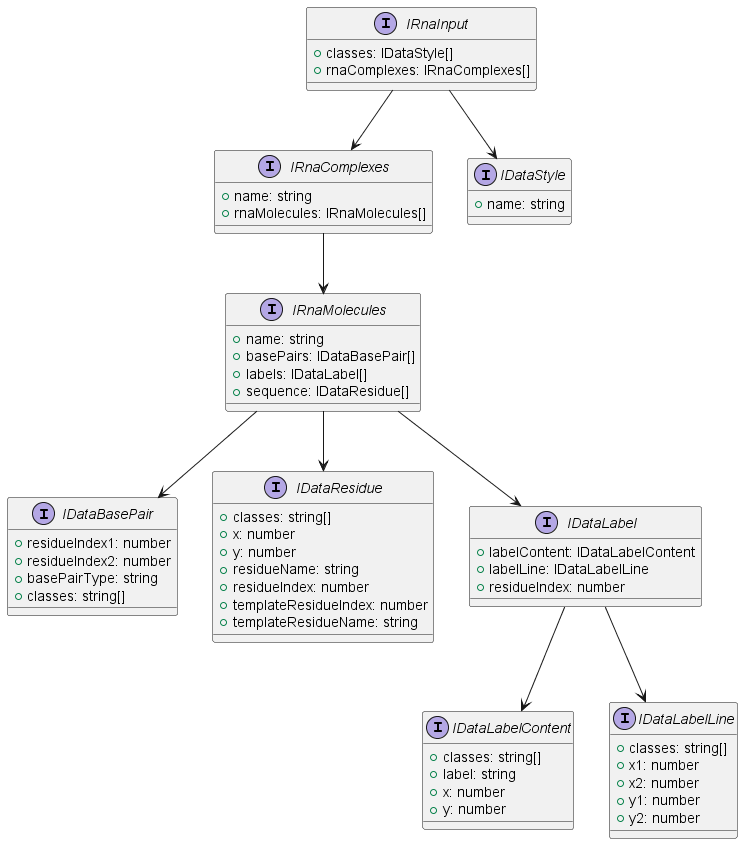
\includegraphics[width=145mm]{../img/rnaInput.png}
  \caption{Interface pro vstupní data}
\end{figure}

\section{Objektový návrh}

\begin{figure}[H]
  \centering
  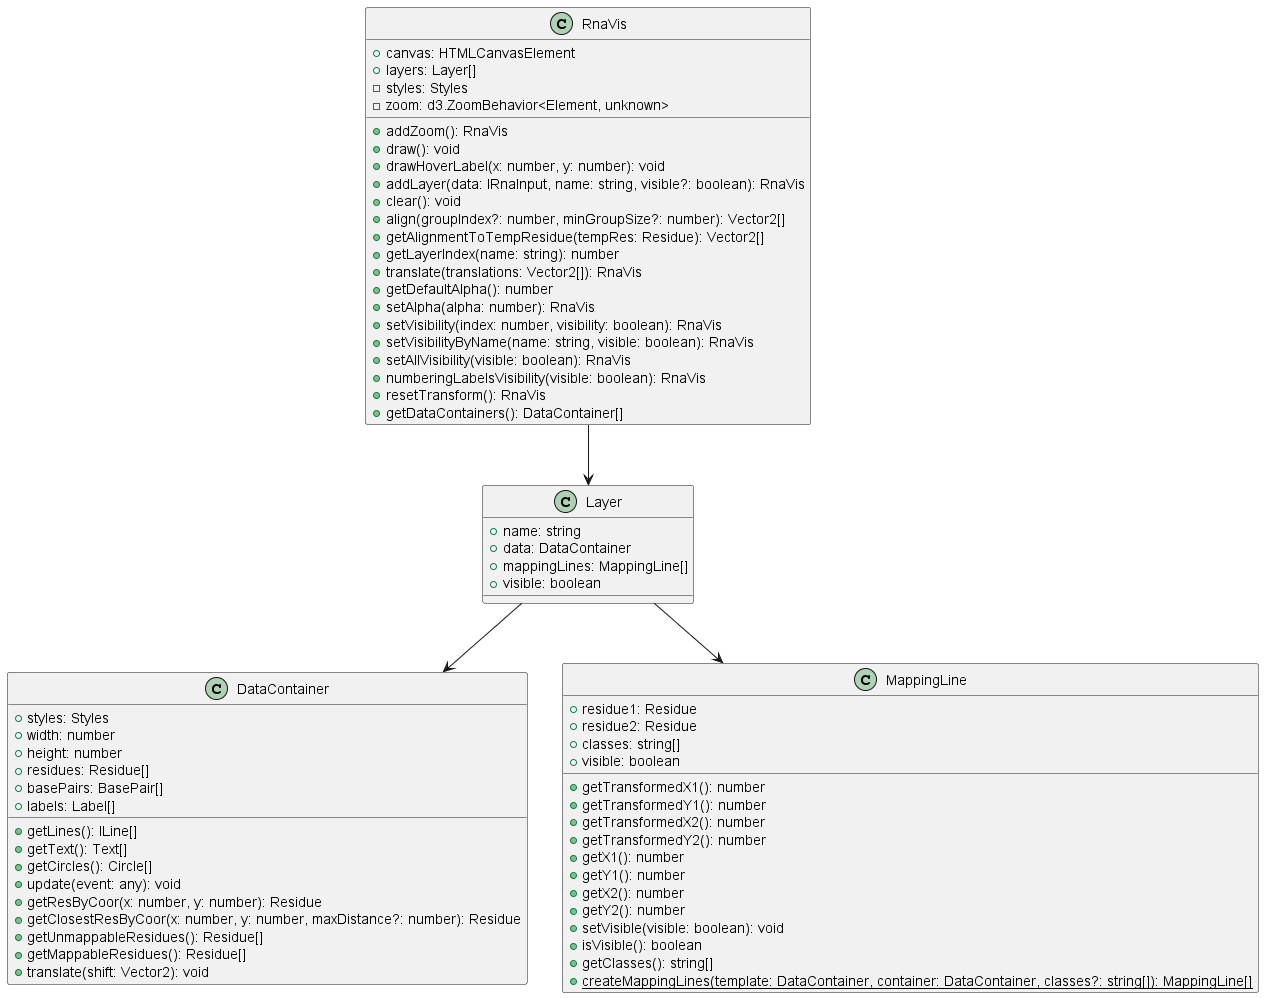
\includegraphics[width=145mm]{../img/rnaVis.png}
  \caption{Interface pro vstupní data}
\end{figure}

\begin{figure}[H]
  \centering
  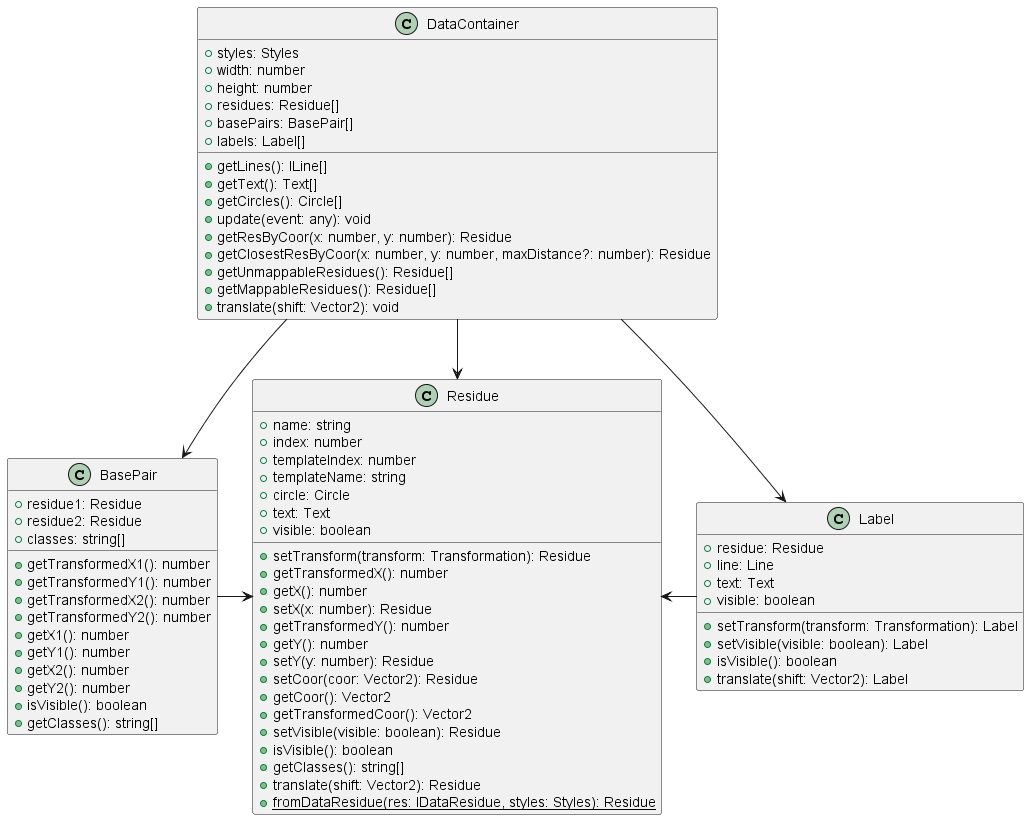
\includegraphics[width=145mm]{../img/dataContainer.png}
  \caption{Interface pro vstupní data}
\end{figure}

\begin{figure}[H]
  \centering
  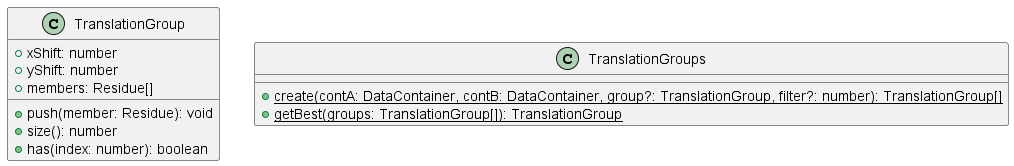
\includegraphics[width=145mm]{../img/translationGroups.png}
  \caption{Interface pro vstupní translationGroups}
\end{figure}

\begin{figure}[H]
  \centering
  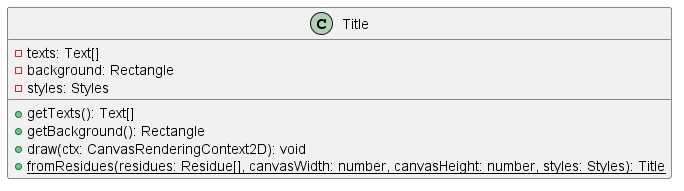
\includegraphics[width=145mm]{../img/title.png}
  \caption{Interface pro vstupní data}
\end{figure}

\begin{figure}[H]
  \centering
  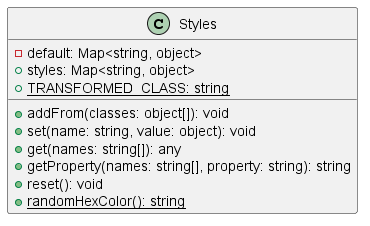
\includegraphics[width=145mm]{../img/styles.png}
  \caption{Interface pro vstupní data}
\end{figure}

\begin{figure}[H]
  \centering
  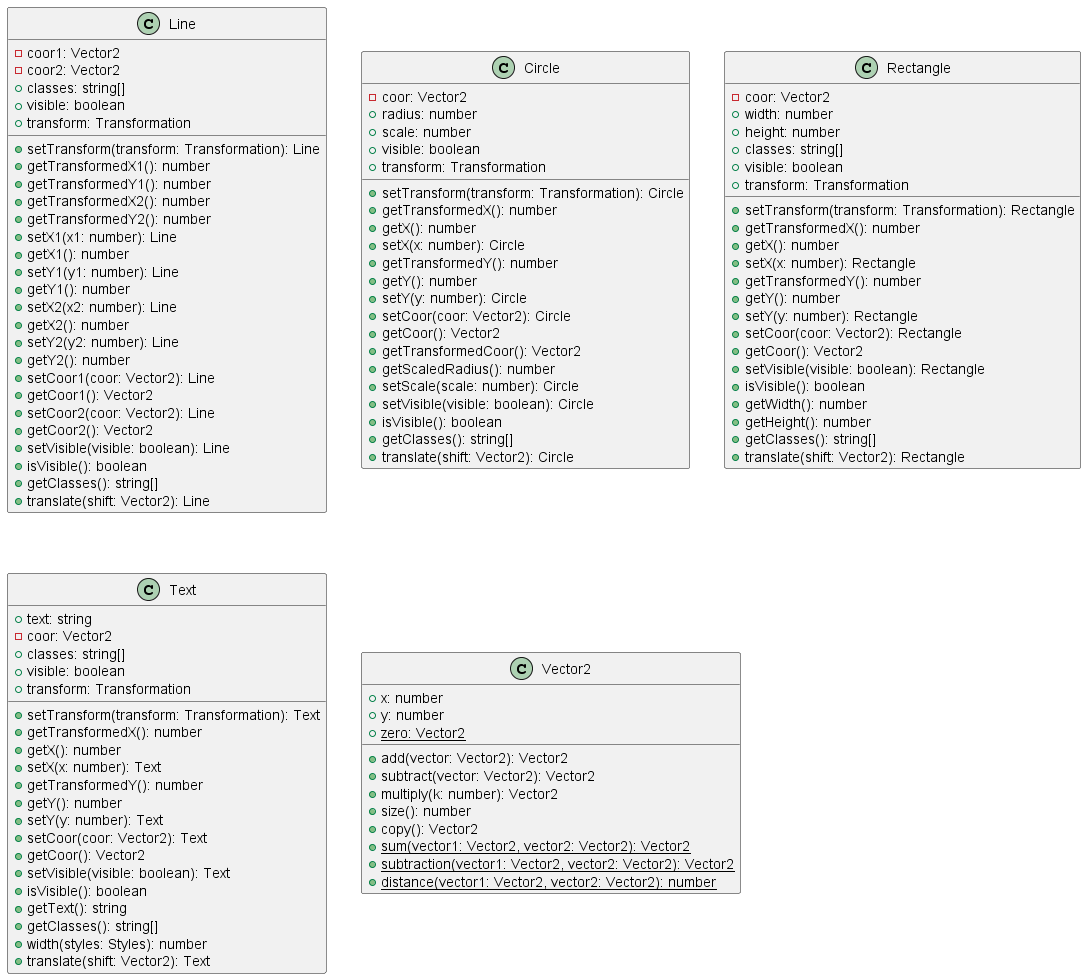
\includegraphics[width=145mm]{../img/primitives.png}
  \caption{Interface pro vstupní data}
\end{figure}

\begin{figure}[H]
  \centering
  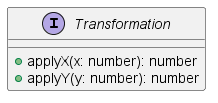
\includegraphics[width=145mm]{../img/iTransformation.png}
  \caption{Interface pro vstupní data}
\end{figure}

\begin{figure}[H]
  \centering
  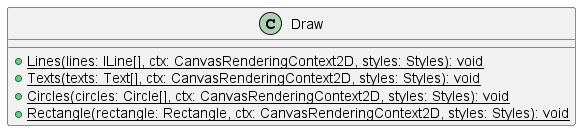
\includegraphics[width=145mm]{../img/draw.png}
  \caption{Interface pro vstupní data}
\end{figure}

\begin{figure}[H]
  \centering
  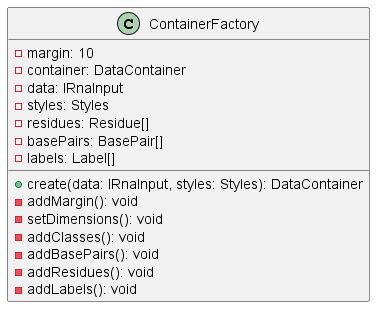
\includegraphics[width=145mm]{../img/containerFactory.png}
  \caption{Interface pro vstupní data}
\end{figure}

\begin{figure}[H]
  \centering
  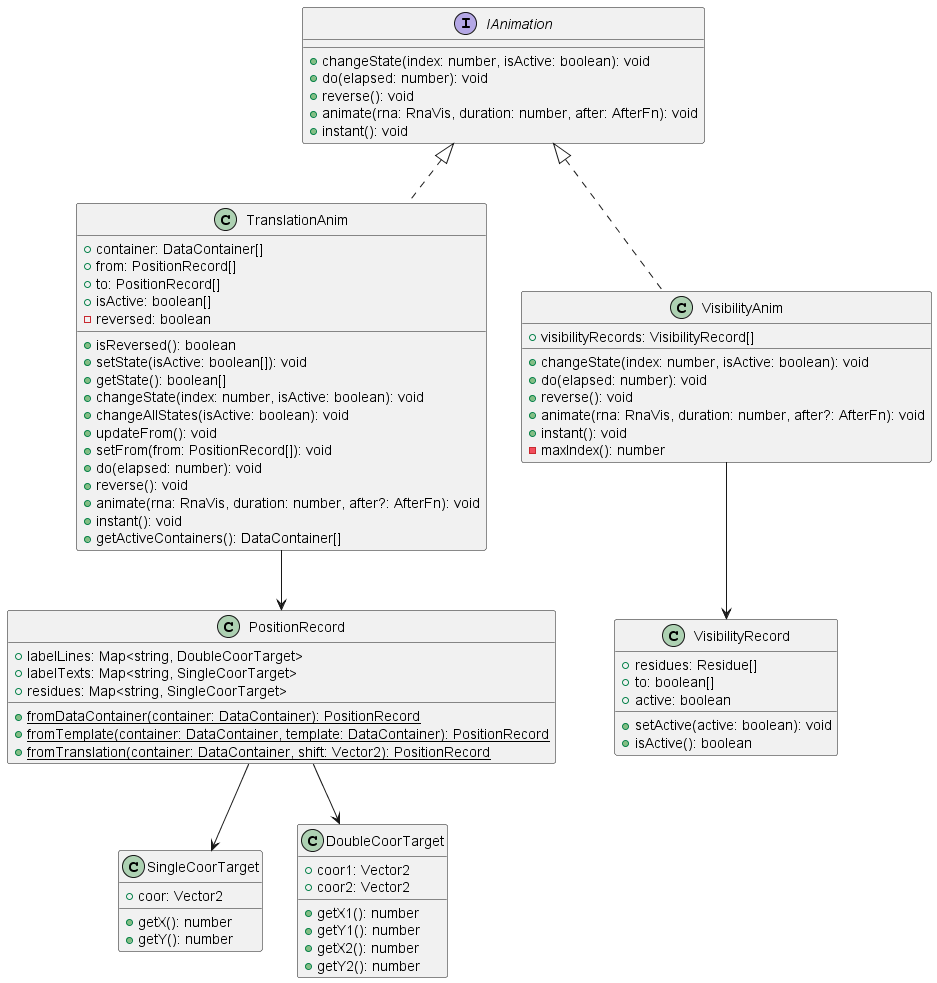
\includegraphics[width=145mm]{../img/animations.png}
  \caption{Interface pro vstupní data}
\end{figure}


